%%
%% This is file `mcmthesis-demo.tex',
%% generated with the docstrip utility.
%%
%% The original source files were:
%%
%% mcmthesis.dtx  (with options: `demo')
%%
%% -----------------------------------
%%
%% This is a generated file.
%%
%% Copyright (C)
%%       2010 -- 2015 by Zhaoli Wang
%%       2014 -- 2019 by Liam Huang
%%       2019 -- present by latexstudio.net
%%
%% This work may be distributed and/or modified under the
%% conditions of the LaTeX Project Public License, either version 1.3
%% of this license or (at your option) any later version.
%% The latest version of this license is in
%%   http://www.latex-project.org/lppl.txt
%% and version 1.3 or later is part of all distributions of LaTeX
%% version 2005/12/01 or later.
%%
%% This work has the LPPL maintenance status `maintained'.
%%
%% The Current Maintainer of this work is Liam Huang.
%%
%%
%% This is file `mcmthesis-demo.tex',
%% generated with the docstrip utility.
%%
%% The original source files were:
%%
%% mcmthesis.dtx  (with options: `demo')
%%
%% -----------------------------------
%%
%% This is a generated file.
%%
%% Copyright (C)
%%       2010 -- 2015 by Zhaoli Wang
%%       2014 -- 2019 by Liam Huang
%%       2019 -- present by latexstudio.net
%%
%% This work may be distributed and/or modified under the
%% conditions of the LaTeX Project Public License, either version 1.3
%% of this license or (at your option) any later version.
%% The latest version of this license is in
%%   http://www.latex-project.org/lppl.txt
%% and version 1.3 or later is part of all distributions of LaTeX
%% version 2005/12/01 or later.
%%
%% This work has the LPPL maintenance status `maintained'.
%%
%% The Current Maintainer of this work is Liam Huang.
%%
\documentclass{mcmthesis}
\mcmsetup{CTeX = false,    % 使用 CTeX 套装时，设置为 true
          tcn = {5049}, problem = \textcolor{red}{A},
          sheet = true, titleinsheet = true, keywordsinsheet = true,
          titlepage = false, abstract = false}
        
\usepackage{newtxtext}     % \usepackage{palatino}
\usepackage[numbers]{natbib}
\usepackage{tocloft}
\usepackage{tabularx}
\usepackage{makecell}
\usepackage{float}
\usepackage{subcaption}
\usepackage{graphicx}
\usepackage{gensymb}
\setlength{\cftbeforesecskip}{6pt}
\renewcommand{\contentsname}{\hspace*{\fill}\Large\bfseries Contents \hspace*{\fill}}

\title{Optimal Power Allocation − Ride to The Future}
% \author{\small \href{http://www.latexstudio.net/}
%   {
\includegraphics[width=7cm]{mcmthesis-logo}}}
\date{\today}

\begin{document}

\begin{abstract}

Who would have thought that the champion of the Tokyo Olympics cycling time trial was a
mathematician? Believe it or not, math does it. In this paper, we will build a mathematical model of
the power curve to help riders win races.


\textbf{In Task 1}, we build a power-duration model based on biological principles. This model has three
stages: Extreme, Severe, Heavy. After substituting the searched rider data into the model, we plot
the power curves of the sprinter and time trial specialist of different genders.


\textbf{In Task 2}, we first use the power curve in \textbf{In Task 1} to build the Human Energy Expenditure
Model, which describes the rider’s constraints on energy limits. We analyzed the dynamic bicycle
model to determine the $P_{out} - v$ relationship during cycling. By analyzing the characteristics of the
track, we establish a piecewise nonlinear programming model with a wide range of applications for
straights, curves, and slopes. For large slope segments or sharp bends, we made detailed calculations
individually. Finally, the optimal output power curves of the riders when riding on the three courses
in Task 1 are solved by Mathematica. The completion times are shown in the table below. Compared
with the champion, our model lags within 6\%, reflecting the model’s accuracy.
\begin{table}[H]
  \centering
  \label{tab:sprint-time}
  \begin{tabular}{lcccc}
    \toprule
    & \multicolumn{2}{c}{Male sprinter} & \multicolumn{2}{c}{Female sprinter} \\
    \cmidrule(lr){2-3} \cmidrule(lr){4-5}
    Course / Region & trial specialist & Self-designed & trial specialist & Self-designed \\
    \midrule
    Time overall & 47.53 & 48.58 & 46.48 & 48.20 \\
    In Japan     & 62.68 & 40.97 & 56.03 & 33.63 \\
    In Belgium   & 58.15 & 59.62 & 53.03 & 54.05 \\
    \bottomrule
  \end{tabular}
\end{table}
\vspace{-0.5cm}
After the model is solved, we perform sensitivity analysis in Task 3 and Task 4. For weather
factors, we focus on the effects of wind speed and direction. When the wind speed changes within
$\pm 2$ m/s and the direction changes within $\pm 180^\circ$, we get the change graph of the output power with
Python. We conclude that the model is robust as its sensitivity to crosswinds is within 1\%. And it
has a 10\% impact on headwinds, which provides us with ideas for team competition strategies.

We also tested the model’s sensitivity to rider deviations. Taking the Belgian track as an example,
we establish the riders’ actual output power function $\overline{P_{out}}$ and add a random disturbance term $\widetilde{P_{out}}$ to
simulate the randomness of the rider. After calculation, the riders can finish the race before they run
out of energy. The time lag is within 2\%.

Inspired by the model’s high sensitivity to headwind, we develop a team time trial strategy in
Task 5. The results are shown in the table below.
\begin{table}[ht]
  \centering
  \label{tab:stage-config}
  \begin{tabular}{lccc}
    \toprule
    Stage & Balance (48\%) & Storage (27\%) & Sprint (25\%) \\
    \midrule
    Formation & Pyramid formation & Linear array & Shield formation \\
    \bottomrule
  \end{tabular}
\end{table}
\vspace{-0.5cm}
Finally, we write to Directeur Sportif with a race guidance for time trial specialists and sprinters.
\begin{keywords}
 power curve, nonlinear programming, dynamics model, formation planning
\end{keywords}

\end{abstract}

\maketitle

%% Generate the Table of Contents, if it's needed.
% \renewcommand{\contentsname}{\centering Contents}
\tableofcontents        % 若不想要目录, 注释掉该句
\thispagestyle{empty}

\newpage

\section{Introduction}

\subsection{Restatement of the Problem}

Cycling is characterized by high power output over a period. This capability can be summarized
by a power curve representing the maximum power a cyclist has generated over time. Due to the
limited endurance of humans, the power curve generally slopes downward to the right, as shown in Figure \ref{fig:power-curve}.

The power curve is used to specify pacing strategies for different courses. And it can prevent
the rider from incurring significant energy losses on impulse. This can be useful in any cycling race
requiring pacing, such as a time trial, Strava segment, or mid-race climb. Using different riding
powers on different road conditions can help riders store energy for sprints and win races.
\begin{figure}[ht]
  \centering
  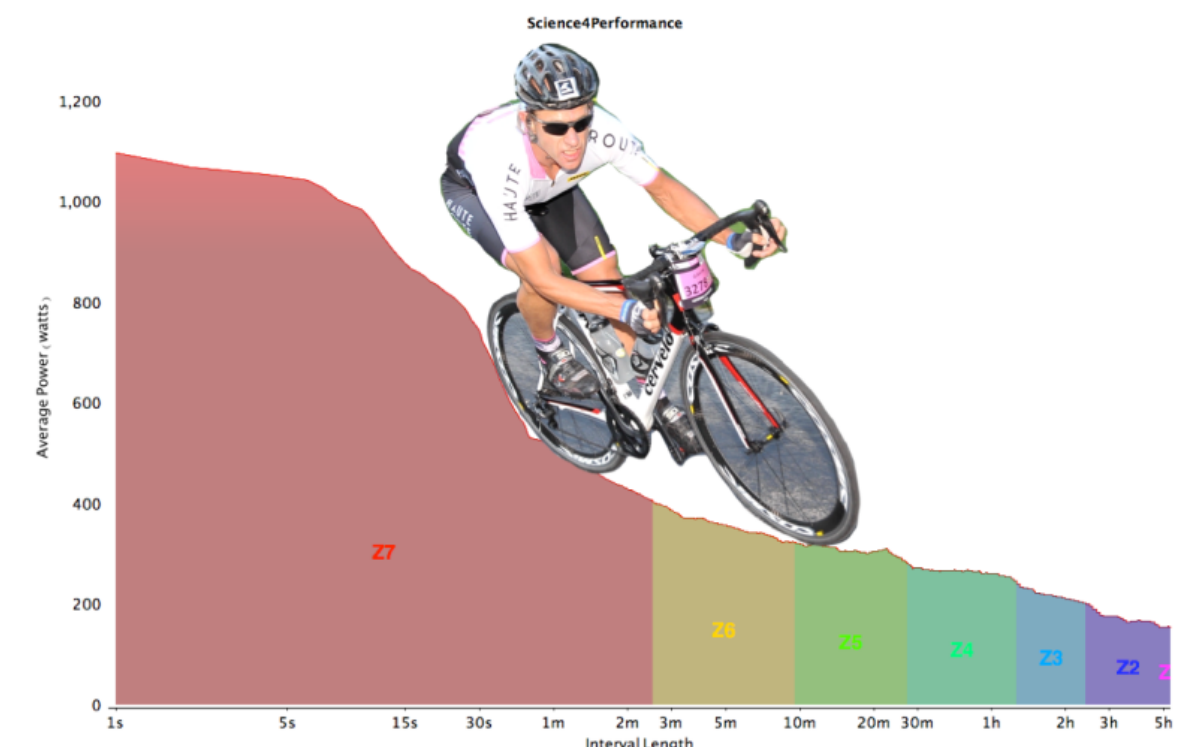
\includegraphics[width=0.5\textwidth]{figures/image1.png}
  \caption{Power curve}
  \label{fig:power-curve}
\end{figure}

We are developing a mathematical model for different types of cyclists. This model is limited
by the total energy a cyclist can expend, focusing on several characteristics of the cyclist, such as
the riding capacity, the position of the rider, and the output power of the rider. Based on the above
understanding, we need to solve the following problems:
\begin{itemize}
\item Define the power curve of a time trial specialist and a sprinter, and consider the genders.
\item Use each power profile defined in Task 1 to apply the model to the following time trial.
    \begin{itemize}
        \item 2021 Olympic Time Trial course in Tokyo, Japan,
        \item 2021 UCI World Championship time trial course in Flanders, Belgium,
        \item At a minimum, a self-designed track that includes at least four sharp turns and a nontrivial
road grade. The end of the course should be near its start point.
    \end{itemize}
\item Determine the model’s sensitivity to weather factors, including wind speed and direction.
\item Analyze how sensitive the results are to rider deviations from the target power distribution.
\item Further, discuss extending the model to a six-player team time trial and get the best results.
Team time is determined by when the fourth rider crosses the finish line.
\item Write a two-page rider’s race guidance for a Directeur Sportif of a team, which should focus
on the result of a time trial course and a rider. It needs to include a model summary and an overview of directions. Readers are people with no mathematical background.
\end{itemize}
\subsection{Literature Review}
Power profiling has always been a scorching area of cycling research. Since the invention of
the power meter in the late 1980s, some researchers have selected a power-duration model that best
describes the training intensity range of athletes. For example, the two-parameter CP model  \cite{Moritani1981CriticalPower} is
only suitable for the severe exercise intensity domain. However, much power output falls within the
high exercise intensity domains. So this model does not provide a fair generalization of the cyclist’s
power curve. This also shows that different examples maybe require different modeling approaches.

With the development of physiology, there has been a growing awareness that a power curve can
be divided into three different exercise intensity domains: Extreme, Severe, and Heavy \cite{Burnley2007OxygenUptake}. And
it provides a comprehensive approach to studying tolerable exercise limits. Previous research has
shown that the anaerobic power reserve (APR) can well predict short-term (<3 min) power outputs
in the extreme exercise intensity domain \cite{Weyand2006SprintPerformance}. In the severe exercise intensity domain, the CP models
are mainly used. There is also a three-parameter CP model \cite{Morton1996ThreeParameterCP}. Currently, a full-power model exists
for the heavy exercise intensity domain \cite{Puchowicz2020OmniDomainPD}.
\subsection{Our Work}
We set up two models based on the assumptions and literature, including the three-stage power
curve and dynamic bicycle models. The power curve model’s three stages are Extreme, Severe,
and Heavy, characterized by distinct human physiological responses. The dynamic bicycle model is
based on physics principles and describes the influence of weather factors on the power output. We
then tested the model on different riders and tracks, with good results. Finally, we designed the team
time trial formation to make our model more applicable.
\begin{figure}[h]
    \centering
    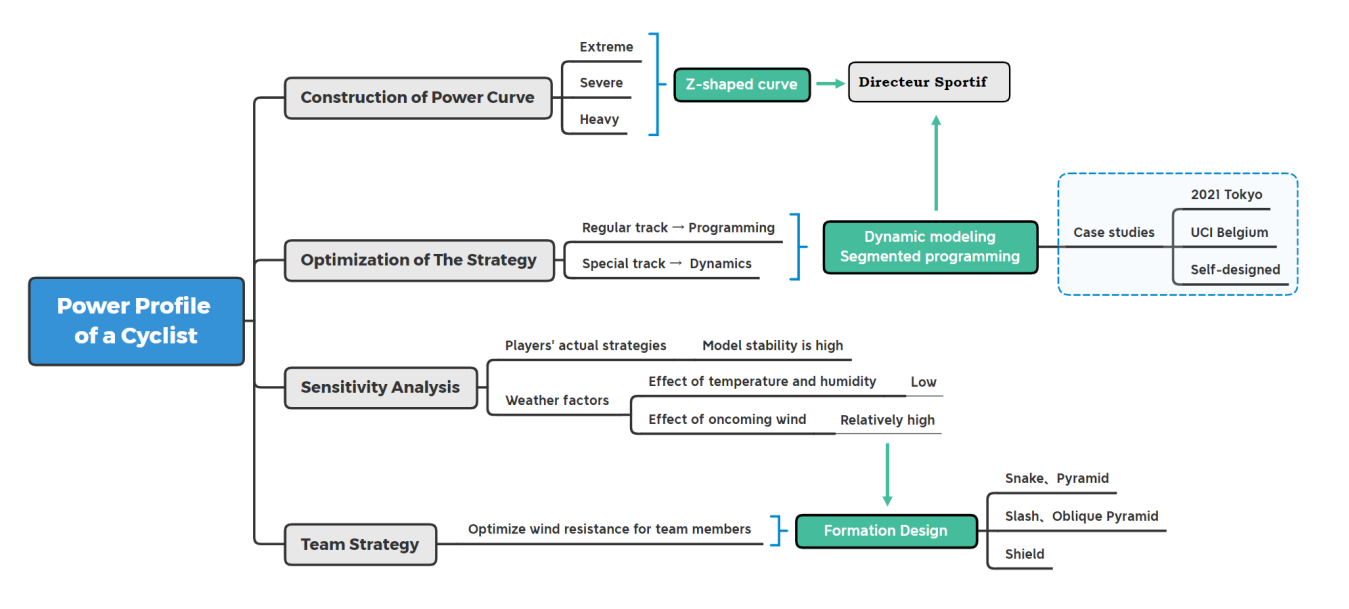
\includegraphics[width=1\textwidth]{figures/image2.png}
    \caption{The structure of our paper}
    \label{fig:structure}
\end{figure}
\section{Assumptions and Justification}
Through a complete analysis of the problem, in order to simplify our model, we make the
following reasonable assumptions.

\noindent \textbf{Assumption 1: Assuming that the temperature and humidity of the cyclist’s competition venue
are suitable, and the fluctuation range is small. Take the temperature range of 67.6 \text{--} 75.6
$^\circ$F and the humidity range of 35.1 \text{--} 45.9\%.}

First, considering that most of the major cycling competitions, including the two cycling competitions given by the problem, are held in July-September. Then check the past weather conditions
and find that the temperature and humidity of the arena are relatively suitable.

\noindent \textbf{Assumption 2: Assuming that cyclists in different physical states, ride with the same power for
the same time, they consume the same amount of energy.}

The principle of physical strength distribution of professional athletes at different stages during
the competition is mostly based on the model of lactic acid accumulation and ATP conversion \cite{Guan2001LacticTraining400m}.
These models have linear properties in explaining human energy expenditure \cite{Wang2007Chinese400m}.

\noindent \textbf{Assumption 3: Assuming that cyclists lose a constant 5\% of their energy during cycling.}

The cyclist is the engine providing the power. Friction in the drive train (chains, gears, bearings,
etc.) causes a small amount of loss, usually around 5\% \cite{Pivit1990DragForce}, assuming the bicycle has a clean and
nicely lubricated drivetrain.
\section{Notations}
The key mathematical notations used in this paper are listed in \autoref{tab:notations}
\vspace{-0.4cm}
\begin{table}[htbp]
\centering
\caption{Notations used in this paper}
\vspace{-0.4cm}
\label{tab:notations}
\begin{tabular}{lll}
\toprule
Symbol & Definitions & Units \\
\midrule
$CP$        & Critical power                                   & $\mathrm{W/kg}$ \\
$W'$        & Work capacity above critical power               & $\mathrm{J/kg}$ \\
$\lambda_E$ & The cyclist's remaining energy / upper energy    & / \\
$P_{\text{out}}$ & The output power of rider                   & $\mathrm{W/kg}$ \\
$t_n$       & Completion time                                  & $\mathrm{s}$ \\
$v_{\text{wind}}$ & Wind speed                                & $\mathrm{m/s}$ \\
\bottomrule
\end{tabular}
\end{table}
\vspace{-0.4cm}
\section{Three stage power-duration models}
As a source of parameters for power curve calculations and track-specific decisions, power profiles
should demonstrate important biological parameters for bike racing of all types of riders. Based
on this premise, we combine the literature review mentioned above to analyze various parameter
characteristics of existing models. In the end, we selecte a sprinter and time trial specialist as our
main subjects. We also calculate the parameters $CP$, $W'$, etc., which can help get the power curve.
,etc., which can help get the power curve.

Next, we obtain the maximum power that can be maintained by different cyclists when they
ride for 5s, 1min, 3min, 5min, 12min, and one has the data source for parameter calcu-lation. We
also consult the relevant website to obtain the calculation method of the Maximum aerobic power
$MAP_{T T F}$ and the value of at the end of every stage.

Finally, we calculated the results and presented the power profile in a tabular format, with a graph
showing the power curves for both athletes of different genders.
\subsection{The Establishment of power-duration model}
First, we use $CP$ to represent the critical power of a cyclist. Critical power means the power
output that cyclists tend to ride at high intensity, usually lasting 30 to 40 minutes. We then use $W'$
to represent the work (in $J/kg$) that the cyclist can expend above $CP$ before fully depleting energy.

Due to the complex metabolism of the human body, and the research on related biomechanics
and biochemical reactions during exercise is also pending breakthroughs. Therefore, the calculation
of $CP$, $W'$
is generally obtained from experimental data. It can be seen from the literature \cite{Bell2021CriticalPowerFTP} that
the calculation formulas of $CP$ and $W'$
are as follows:
\begin{equation}
    CP = \frac{12 \cdot P_{12} - 3 \cdot P_{3}}{9}
\end{equation}
\begin{equation}
    W' = 0.24s \cdot \left( P_{3} - P_{12} \right)
\end{equation}
where $P_3$ is the average power of a cyclist who rides hard for three minutes divided by his mass,
while $P_{12}$ is the same as $P_3$ but for 12 minutes.And we also have the formulas of $MAP_{T T F}$
\begin{equation}
    MAP_{TTF} = \frac{W'}{P - CP} + \frac{W'}{P_{\max} - CP}
\end{equation}
where $P_{\max}$ is ultimate power. According to relevant information \cite{Bell2021CriticalPowerFTP}, we estimate that $P_{\max} \approx P_{5s}$.
Integrating the formulas above, we get the following table:
\begin{table}[ht]
  \centering
  \caption{The power profile of different types of riders I}
  \label{tab:power_profile_I}
  \vspace{-0.4cm}
  \begin{tabular}{ccccccc}
    \toprule
    Race & Gender & 5s & 1min & 3min & 5min & 12min \\
    \midrule
    Sprinter & M & 21.03 & 9.09 & 6.95 & 4.81 & 4.70 \\
     & F & 16.40 & 7.39 & 6.17 & 4.17 & 4.13 \\
    Time Trial Specialist & M & 16.89 & 8.74 & 7.14 & 5.53 & 5.46 \\
     & F & 13.39 & 7.11 & 5.85 & 4.83 & 4.75 \\
    \bottomrule
  \end{tabular}
\end{table}
\vspace{-0.5cm}
\begin{table}[ht]
  \centering
  \caption{The power profile of different types of riders II}
  \vspace{-0.4cm}
  \label{tab:power_profile_II}
  \begin{tabular}{ccccccc}
    \toprule
    Race & Gender & FTP & CP & W' & MAP$_{TTF}$ & CP$_{TTF}$ \\
    \midrule
    Sprinter & M & 3.91 & 3.94 & 0.54 & 1.10 & 33.79 \\
     & F & 3.39 & 3.45 & 0.49 & 0.99 & 32.60 \\
    Time Trial Specialist & M & 4.98 & 4.90 & 0.40 & 0.97 & 40.29 \\
     & F & 4.38 & 4.38 & 0.26 & 0.92 & 34.41 \\
    \bottomrule
  \end{tabular}
\end{table}


According to the different exercise time and the characteristics of various athletes in different
stages, we refer to the literature review to solve the power curve in three stages. Its scope and
calculation model are shown in the following table:
\begin{table}[H]
\centering
\caption{Three stage power-duration models}
\vspace{-0.4cm}
\label{tab:power_model}
\small
\begin{tabularx}{\textwidth}{l>{\raggedright\arraybackslash}p{3.5cm}Xl}
\hline
Stage & Model & Equation & Range \\
\hline
I.Extreme & Anaerobic power reserve & $P_{(t)} = P_3 + (P_{\max} - P_3) \cdot e^{-kt}$ & $t < MAP_{TTF}$ \\

II.Severe & 2-parameter critical power model & $P_{(t)} = \frac{W'}{t} + CP$ & \makecell[l]{$t > MAP_{TTF}$ \\ $t < CP_{TTF}$} \\

III.Heavy & Omni power duration model & $P_{(t)} = \frac{W'}{t} \cdot \left(1 - e^{t \cdot \frac{CP-P_{\max}}{W'}}\right) + CP - A \cdot \ln\left(\frac{t}{CP_{TTF}}\right)$ & $t > CP_{TTF}$ \\
\hline
\multicolumn{4}{l}{(Combining curve continuity, take k=0.7, A=0.1)} \\
\end{tabularx}
\end{table}
\subsection{The Solution of Power-Duration Model}
Then we combine formula (1), formula (2) and the data in Table \ref{tab:power_profile_I} together with the data in Table
\ref{tab:power_profile_II}, and substitute them into the formula in Table \ref{tab:power_model}. We use Mathematica to calculate and draw the
curve to get the following power curve in Figure \ref{fig:main}.
\begin{figure}[ht]
  \centering
  \begin{subfigure}[b]{0.3\textwidth}
    
\includegraphics[width=\textwidth]{image3_1.png}
    \caption{ Power curve for 0-40 min}
    \label{fig:sub1}
  \end{subfigure}
  \hfill
  \begin{subfigure}[b]{0.3\textwidth}
    
\includegraphics[width=\textwidth]{image3_2.png}
    \caption{Power curve for 0-1 min(Extreme domain)}
    \label{fig:sub2}
  \end{subfigure}
  \hfill
  \begin{subfigure}[b]{0.3\textwidth}
    
\includegraphics[width=\textwidth]{image3_3.png}
    \caption{Power curve for 1-40 min(Severe and Heavy domain)}
    \label{fig:sub3}
  \end{subfigure}
  \caption{The power curve of different types of rider}
  \label{fig:main}
\end{figure}
\vspace{-0.4cm}

Looking at the curves, in the same event, the power curve of male cyclists is always above the
power curve of female cyclists. This is consistent with the pattern of better physical strength in male
cyclists. In addition, in terms of short bursts ($t < 1s$), the power of the sprinter was significantly
higher than that of the time trial specialist. In the middle- and long-distance riding competitions, the
time trial specialist are better.
\section{Piecewise Nonlinear Programming for Time Trial}
\subsection{The Establishment of Human Energy Expenditure Model}
As To apply the power curve model established in Task 1 to the courses, we next derive a human
energy expenditure model suitable for the problem background.

Let $m \cdot P_{out}$ be the power output by the cyclist at time t, where $m$ is the weight of the cyclist, and
$P_{out}$ is the output power per unit mass of the cyclist.
\begin{figure}[H]
  \centering
  \begin{subfigure}[b]{0.3\textwidth}
    
\includegraphics[width=\textwidth]{image4_1.png}
    \caption{ The schematic diagram of variable power output}
    \label{fig:sub1}
  \end{subfigure}
  \hfill
  \begin{subfigure}[b]{0.3\textwidth}
    
\includegraphics[width=\textwidth]{image4_2.png}
    \caption{The discrete function of $P_{out} - t$}
    \label{fig:sub2}
  \end{subfigure}
  \hfill
  \begin{subfigure}[b]{0.3\textwidth}
    
\includegraphics[width=\textwidth]{image4_3.png}
    \caption{The continuous function of $P_{out} - t$}
    \label{fig:sub3}
  \end{subfigure}
  \caption{The illustration of Task 2}
  \label{fig:The illustration of Task 2}
\end{figure}

According to Assumption 2, we calculate in proportion to the total energy consumed. For the
power discrete values shown in the middle of Fig\ref{fig:The illustration of Task 2}, the ratio of the cyclist’s remaining energy to the
upper energy limit is expressed as follows:
\begin{equation}
    \lambda_E = \frac{E_R}{E_m} = 1 - \sum_i \frac{\Delta t_i}{T_i}
\end{equation}
where $T_i$ is the longest holding time of the current power when the body is full of energy. In the
middle of fig\ref{fig:The illustration of Task 2}, the result of $λ_E$ is $λ_E = 1 −
\frac{10s}{20s} −\frac{5s}{10s} = 0$.

However, when solving practical problems, it is impossible for cyclists to strictly follow a detailed
plan of the optimization solution. This can lead to cyclists hitting their fitness limits before they
finish the race. Therefore, we reduce the 1 on the right side of the equation to 0.95, leaving 5\% of
the remaining stamina to deal with the above situation.

Change the discrete model to continuous. For the continuity \( P_{out}(t) \) shown in the right of fig. \ref{fig:The illustration of Task 2}, cut an approximate rectangle with a width of \( dt \), and the height of the rectangle is \( T(P_{out}) \). Next, replace the summation with the integral to get the formula for \( \lambda_E \) at time \( t \)
\begin{equation}
\lambda_E(t) = 1 - \int_0^t \frac{d\tau}{T(P_{out}(\tau))}
\end{equation}
where \( T(P) \) is the inverse function of the power curve expression \( P(t) \), i.e., \( T(P) = P^{-1}(P) \).


If the cyclist just uses up his energy when he reaches the finish line, the following constraint exists:
\begin{equation}
1 - \lambda_E(t) = \int_0^t \frac{d\tau}{T(P_{out}(\tau))} = 1
\end{equation}

However, when solving practical problems, it is impossible for cyclists to strictly follow a detailed
plan of the optimization solution. This can lead to cyclists hitting their fitness limits before they
finish the race. Therefore, we reduce the 1 on the right side of the equation to 0.95, leaving 5\% of
the remaining stamina to deal with the above situation.
\subsection{The Mathematical Relationship Between Power Output And Speed}
We conduct a dynamic analysis on the bicycle, the force diagram is shown in the fig.\ref{fig:5sub1}, and the following formula is established:
\begin{equation}
F_{\text{total}} = \left( F_{\text{roll}} + F_{\text{slope}} + F_{\text{accel}} + F_{\text{wind}} \right) / \eta 
\end{equation}
where \( F_{\text{total}} \) is the athlete's active force, \( F_{\text{roll}} \) is the rolling friction force, \( F_{\text{accel}} \) is the inertial force generated by the acceleration, \( F_{\text{wind}} \) is the aerodynamic resistance, and \( F_{\text{slope}} \) is the slope resistance.
(negative value when going downhill). According to assumption 3, we set \(\eta\) as the driving efficiency,
which is 95\%.
\begin{figure}[H]
  \centering
  \begin{subfigure}[b]{0.45\textwidth}
    
\includegraphics[width=\textwidth]{image5_1.png}
    \caption{Analysis of bicycle force}
    \label{fig:5sub1}
  \end{subfigure}
  \hfill
  \begin{subfigure}[b]{0.45\textwidth}
    
\includegraphics[width=\textwidth]{image5_2.png}
    \caption{$P_{out} - v$ plot}
    \label{fig:5sub2}
  \end{subfigure}
  \label{fig:5}
  \vspace{-0.8cm}
  \caption{  }
\end{figure}
According to the principles of physics, the calculation formulas of various physical quantities are as follows:
\begin{equation}
F_{\text{roll}} = C_r \cdot M g \quad (0.0015 < C_r < 0.015, M = m + m_{\text{bike}} \approx 1.2 \cdot m)
\end{equation}
\begin{equation}
F_{\text{slope}} = M g \cdot \sin \theta
\end{equation}
\begin{equation}
F_{\text{accel}} = a \cdot M
\end{equation}
\begin{equation}
F_{\text{wind}} = \frac{1}{2} C_W A \cdot \rho v_{\text{wind}}^2
\end{equation}
where \( \rho \) is the air density. Based on the temperature and humidity values in Assumption 1, we get \( \rho = 1.29 \, \text{kg/m}^3 \). \( C_W \) is the wind resistance coefficient. \( A \) is the frontal area, which satisfies \( C_W A = 0.39 \, \text{m}^2 \) and is only valid for the frontal incident flow. Under no wind conditions, \( v_{\text{wind}} = v_{\text{bike}} \).

Combining the above equations, and then by \( m \cdot P_{\text{out}} = F_{\text{total}} \cdot v \), we can obtain the conversion relationship between \( P_{\text{out}} \) and \( v \), as shown in the right of fig. 5.
\subsection{The Racing Strategy of Self-designed course}
We first design a course that includes basic road conditions such as straights, downhill slopes,
and sharp turns to obtain the strategies to be adopted in different road conditions. This strategy is
then used to solve complex course problems in two real races.
\begin{figure}[H]
\centering
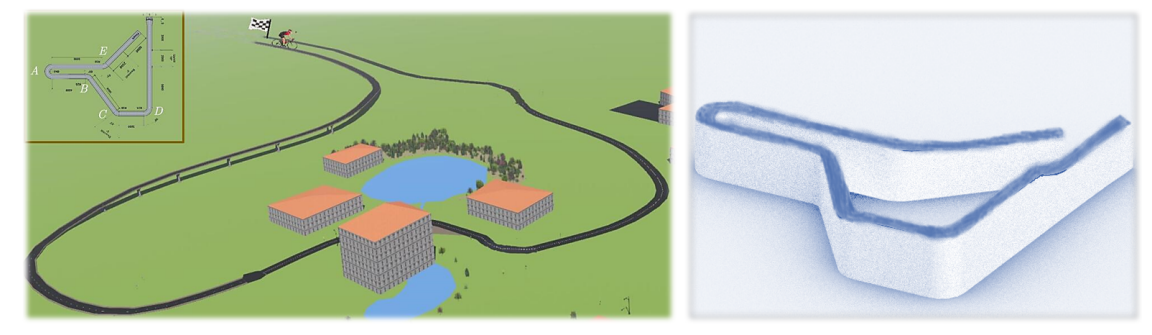
\includegraphics[width=0.8\textwidth]{figures/image6.png}
\caption{ Left: Self-designed track scene construction. Right: Self-designed 3D map of the track}
\label{fig:6}
\end{figure}
\vspace{-0.5cm}
We use Webots software to build the track scene,
 and draw the plan and 3D map of the selfdesigned course, 
 as shown in fig.\ref{fig:6}. Section AB is a short uphill,
  section CD is a long uphill and
section EF is a long downhill.
\subsubsection{Analysis of Riding Strategies on Curved Roads}
We set the inner diameter of the curve as \( r \), the road width as \( d \), and \( R \) as the radius of the optimal path arc. According to the centripetal force calculation formula \( F = \frac{mv^2}{r} \), the maximum turning rate can be achieved by taking the route shown in the figure below. In this case, the physical quantities are related as follows:
\begin{figure}[H]
    \centering
    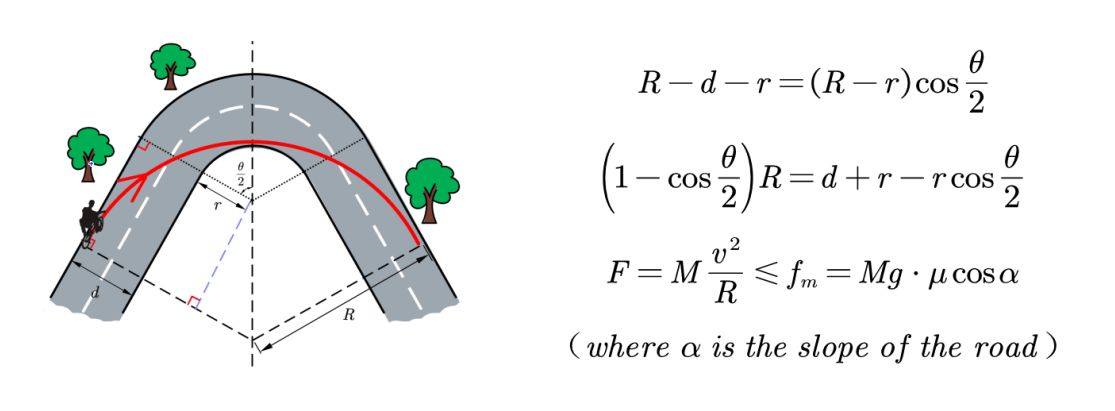
\includegraphics[width=0.8\textwidth]{figures/image.png}
\end{figure}
Integrating, we get the maximum speed of cornering
\begin{equation}
    v_{\max} = \sqrt{\frac{\mu g \cdot \cos \alpha \cdot \left[ d + r - r \cos \frac{\theta}{2} \right]}{1 - \cos \frac{\theta}{2}}} \tag{*}
\end{equation}
Since the total length of the curves of the self-designed track is 0.185km, it can be ignored
compared with the total length of the straight track of 36.5km. Therefore, we first only consider
the straight time when calculating the time and ignore the speed change problem in the turn. We
approximated the rider’s power output before and after the turn as a step change. After this is done,
we complete the optimal passing scheme for each turn.
\subsubsection{Analysis of Straight Riding Strategy}
Next, we analyze the straight riding strategy. We assume that there are \( n_i \) sections of horizontal straights (lengths \( L_1, L_2, ..., L_{n_i} \)), \( n_j \) sections of downhill straights (lengths \( D_1, D_2, ... D_{n_j} \)) and \( n_k \) sections of uphill straights (lengths \( U_1, U_2, ..., U_{n_k} \)). The conversion function \( v - P_{\text{out}} \) of the horizontal straight is \( v^{(\text{straight})}(P) \), the function for a downhill straight with an inclination angle \( \theta_j \) is \( v_{\theta_j}^{(\text{downhill})}(P) \), and \( v_{\theta_k}^{(\text{uphill})}(P) \) is the function for a uphill straight with an inclination angle \( \theta_k \). The task then turns into the following planning problem:
\begin{equation}
\begin{aligned}
t &= \sum_{i=1}^{n_i} \frac{L_i}{v^{(\text{straight})}(P_i)} + \sum_{j=1}^{n_j} \frac{D_j}{v_{\theta_j}^{(\text{downhill})}(P_j)} + \sum_{k=1}^{n_k} \frac{U_k}{v_{\theta_k}^{(\text{uphill})}(P_k)} \\
find \indent P_{\text{out}}(t), \\
\min \{ t \} \quad \text{s.t.} \quad & \int_0^{t_n} \frac{dt^*}{T \left( P_{\text{out}} \left( t^* \right) \right)} = 0.95
\end{aligned}
\end{equation}

In this map, \( n_i = 7, n_j = 1, n_k = 1 \). The subscript of \( L, D, U \) is marked in an increasing manner from the start point to the end point.

As for this function, we discretize \( P_{\text{out}}(t) \). 
This makes the numerical calculation of 
$\int_0^{t_n} \frac{dt^*}{T(P_{\text{out}}(t^*))} $
easier to implement. And we can use \( P_i, P_j, P_k \) to draw the \( P_{\text{out}}(x) \) graph, which is more helpful for cyclists to judge the output power according to the track landscape.
\begin{figure}[ht]
  \centering
  \begin{minipage}{0.45\textwidth}
    \centering
    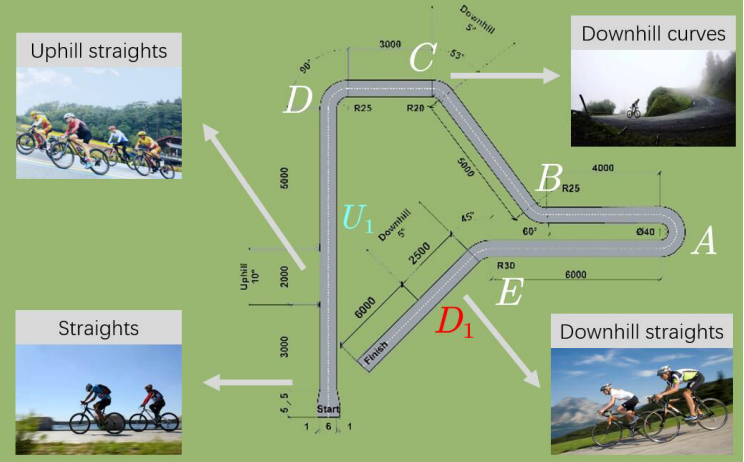
\includegraphics[width=\textwidth]{figures/image7.png}
    \caption{Ramp division}
    \label{fig:image7}
  \end{minipage}\hfill
  \begin{minipage}{0.45\textwidth}
    \centering
    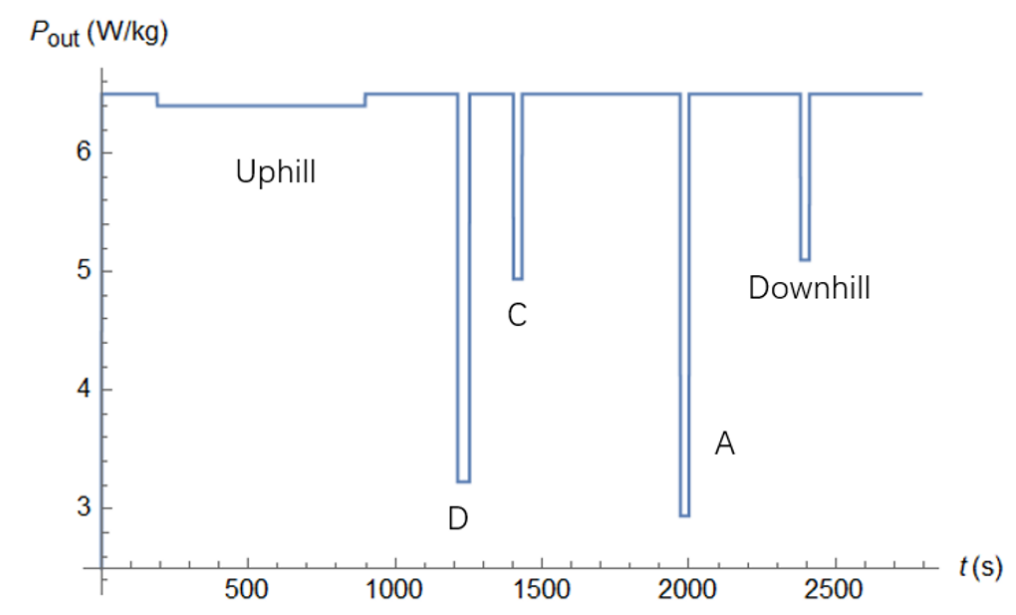
\includegraphics[width=\textwidth]{figures/image8.png}
    \caption{ Time trial male rider strategy}
    \label{fig:image8}
  \end{minipage}
\end{figure}

We use Mathematica to numerically solve the inverse function and the nonlinear programming
function Minimize. Then get the results shown in the table below:
\begin{table}[ht]
  \centering
  \caption{The results of the self-designed time trial course}
  \vspace{-0.4cm}
  \begin{tabular}{@{}cccccc@{}}
    \toprule
    Rider type & Gender & $P_{\text{out}}(L)$ & $P_{\text{out}}(U_1)$ & $P_{\text{out}}(D_1)$ & $t$ \\
    \midrule
    Sprinter & M & 6.0 & 6.3 & 5.2 & 47.53min \\
             & F & 5.8 & 6.0 & 5.1 & 48.58min \\
    Time Trial Specialist & M & 6.5 & 6.4 & 5.1 & 46.48min \\
                         & F & 6.0 & 5.9 & 5.0 & 48.20min \\
    \bottomrule
  \end{tabular}
    \label{tab:time_trial_results}
\end{table}

We next solve for the turn time. We use the formula (*) and the conversion function to solve, and
get the following results:  \vspace{-0.4cm}
\begin{table}[ht]
  \centering
  \caption{The results of each turn}
  \vspace{-0.4cm}
  \begin{tabular}{@{}clcccc@{}}
    \toprule
    Curve number & A & B & C & D & E \\
    \midrule
    $P_{\text{out}}$ & 2.94 & 7.27 & 4.94 & 3.23 & 12.13 \\
    $v$ & 7.34 & 11.02 & 9.48 & 7.98 & 13.38 \\
    \bottomrule
  \end{tabular}
    \label{tab:turn_results}
\end{table}

Comparing the above two tables, it can be seen that the cyclist must slow down to pass the turn
due to the large angle of turns A and D. Although the turn at C is 53 degrees, it is on a scope, which
reduces the upper limit of static friction. So deceleration is also required. Turn B is no need to slow
down.

In bicycle competition, the acceleration can reach $2m/s^{2}$ when accelerating and decelerating.
The time for this process can be ignored.

Combining the results of the straights and corners above, the optimal $P_{\text{out}}(t)$ during the rider’s
competition is shown in fig. \ref{fig:image8} (taking a male time trial specialist as an example).

\subsection{The Strategy of 2021 UCI World Championship time trial course}
\begin{figure}[ht]
  \centering
  \begin{minipage}{0.45\textwidth}
    \centering
    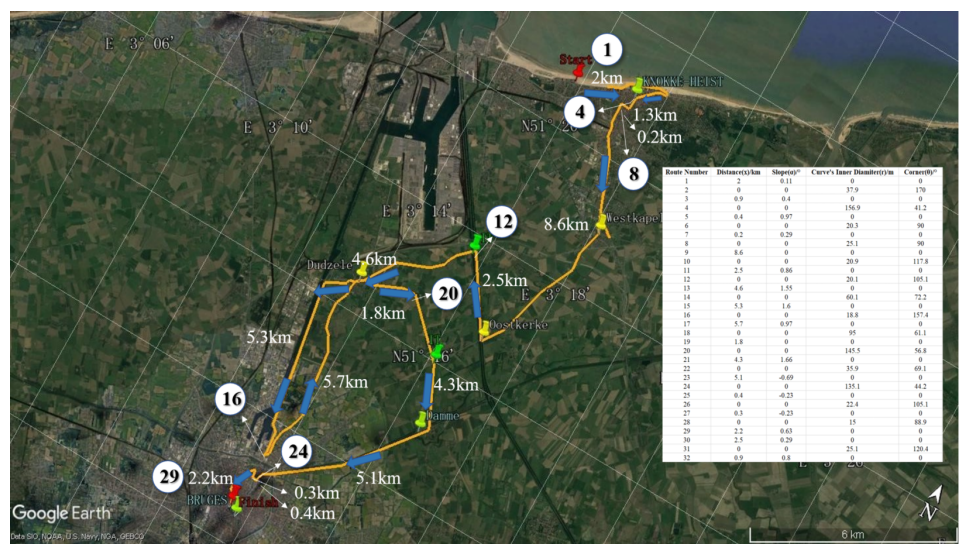
\includegraphics[width=\textwidth]{figures/image9.png}
    \caption{ 2021 UCI Track Division}
    \label{fig:image9}
  \end{minipage}\hfill
  \begin{minipage}{0.45\textwidth}
    \centering
    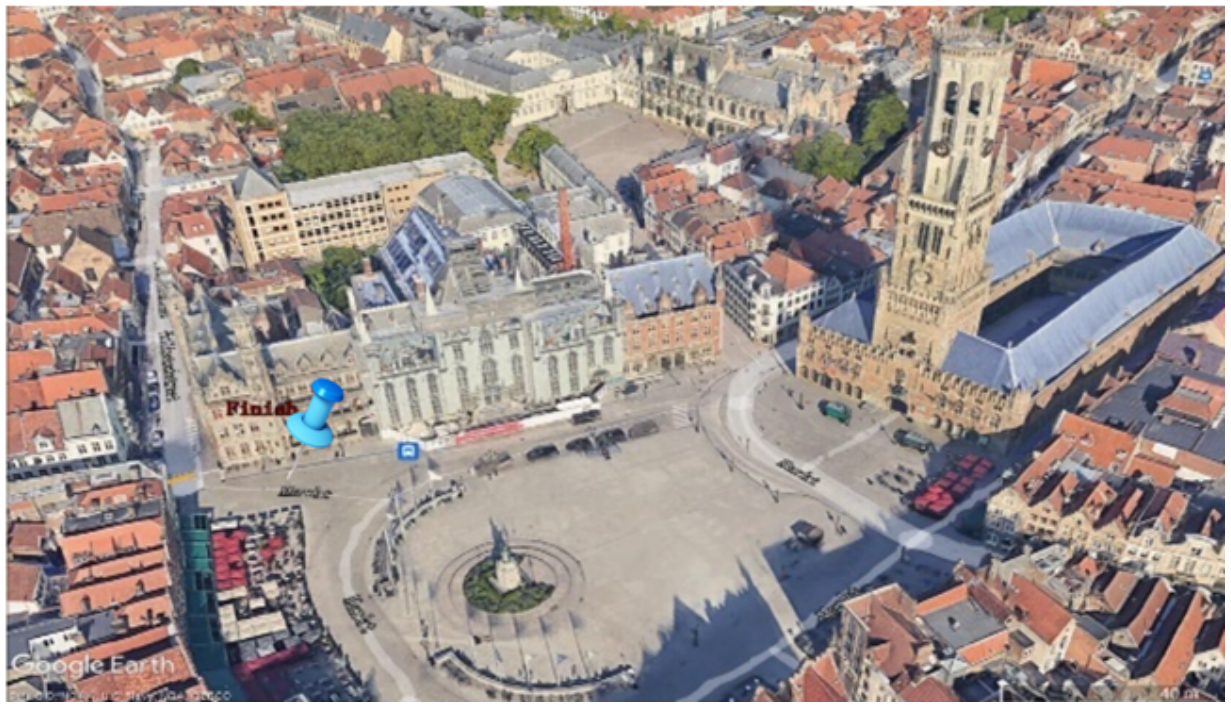
\includegraphics[width=\textwidth]{figures/image10.png}
    \caption{The finish near the city center plaza}
    \label{fig:image10}
  \end{minipage}
\end{figure}
According to the data on UCI’s official website, we determined the terrain and route characteristics
of the area of the course on Google Earth. And we divide the track into 32 parts by analyzing the
similarities and differences of the road sections (as shown in fig. \ref{fig:image9}). Among them, 15 sections are
curves, 2 sections are horizontal straights, 3 sections are downhill straights, and 12 sections are uphill
straights.
\begin{figure}[H]
    \centering
    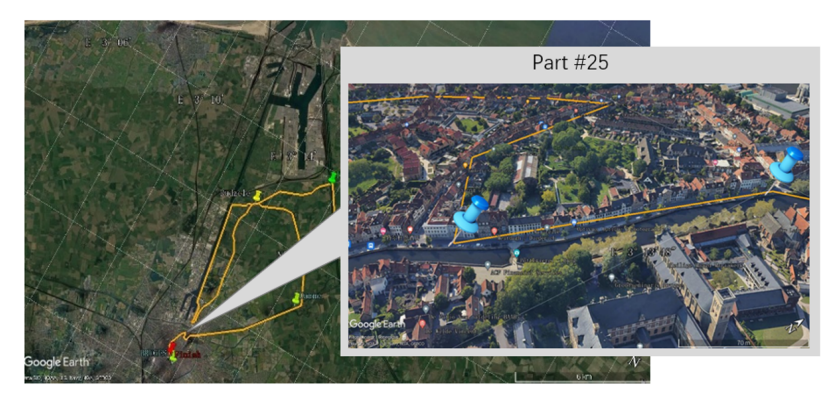
\includegraphics[width=0.8\textwidth]{figures/image11.png}
    \caption{Detail of section \#25}
    \label{fig:image11}
\end{figure}
It is worth noting that the competition area is located in northwestern Belgium. It is in the
High Flanders Plain with small undulations. The maximum slope angle in the uphill section of this
area is \(1.66^\circ\), while in the downhill section is \(0.69^\circ\). Besides, there are sufficiently long straights to
transition between adjacent turns. The shortest straight is our section numbered 25 (shown in fig. \ref{fig:image11}
). Section \#25 is about 400m long, which is enough for cyclists to maintain the optimum for a long
time. Therefore, the rider’s passing time is hardly affected by turning, and the piecewise discrete
programming model is still applicable.
Different from the Olympic Time Trial course in Tokyo, this competition has relatively low
requirements on players’ driving skills and cornering skills and focuses on physical distribution and
endurance.
\subsubsection{The Strategy of Straight and Ramp Riding in Belgium course}
Based on the above analysis, we can still use the method of self-designed track. First, we solve
the straight strategy, as follows:
\begin{equation}
\begin{gathered}
t=\sum_{i=1}^{n_i}\frac{L_i}{v^{(\text{straight})}(P_i)}
 +\sum_{j=1}^{n_j}\frac{D_j}{v^{(\text{downhill})}_{\theta_j}(P_j)}
 +\sum_{k=1}^{n_k}\frac{U_k}{v^{(\text{uphill})}_{\theta_k}(P_k)}\\[4pt]
\text{find }P_{\text{out}}(t),\quad
\min\{t\}\quad\text{s.t.}\quad
\int_0^{t_n}\frac{dt^*}{T\!\bigl(P_{\text{out}}(t^*)\bigr)}=0.95
\end{gathered}
\end{equation}



where $n_i = 2$, $n_j = 3$, $n_k = 12$.


Considering that there are many uphill sections and different slope angles. It makes the model
difficult to converge, which is extremely unfavorable for the computer’s nonlinear programming
solution. Due to the small undulating terrain in this area, we selected 9 road sections with slope
angles below \(1^\circ\)
(\#1, 3, 5, 7, 11, 17, 29, 30, 32) and group them together. Then we can weight the
slope angle according to the road length to get the integrated new slope. We next use the new slope
to solve.

Since $\sin\theta$ is approximately linear in the range of small slope angles, when integrating multiple ramps, we can use approximately linear properties for weighting. The parameters are determined by the following equations:
\begin{align}
U_{c} &= \sum_{k\in\mathcal{A}_{U}} w_{k}\,U_{k}, \quad \theta_{c}= \sum_{k\in\mathcal{A}_{U}} w_{k}\,\theta_{k}, \label{eq:14}\\[2pt]
w_{k} &= \frac{U_{k}}{\sum_{q\in\mathcal{A}_{U}} U_{q}}. \label{eq:15}
\end{align}

After processing, the problem is transformed into the following nonlinear programming problem:
\begin{align}
t &= \sum_{i=1}^{n_i}\frac{L_i}{v^{(\text{straight})}(P_i)} + \sum_{j=1}^{n_j}\frac{D_j}{v^{(\text{downhill})}_{\theta_j}(P_j)} + \sum_{k=1}^{n_k}\frac{U_k}{v^{(\text{uphill})}_{\theta_k}(P_k)} + \frac{U_c}{v^{(\text{uphill})}_{\theta_c}(P_c)}\notag \\[4pt]
&\quad\text{find }P_{\text{out}}(t),\\[2pt]
&\quad\min\{t\}\quad\text{s.t.}\quad \int_0^{t_n}\frac{dt^*}{T\!\bigl(P_{\text{out}}(t^*)\bigr)}=0.95 \notag
\end{align}

\begin{figure}[H]
  \centering
  \begin{subfigure}[b]{0.3\textwidth}
    
\includegraphics[width=\textwidth]{image12_1.png}
    \caption{ $P_{out}(x)$ plot for
sprinters}
    \label{fig:12sub1}
  \end{subfigure}
  \hfill
  \begin{subfigure}[b]{0.3\textwidth}
    
\includegraphics[width=\textwidth]{image12_2.png}
    \caption{$P_{out}(x)$ plot for time trial specialist}
    \label{fig:12sub2}
  \end{subfigure}
  \hfill
  \begin{subfigure}[b]{0.3\textwidth}
    
\includegraphics[width=\textwidth]{image12_3.png}
    \caption{Scatter plot of maximum rate in the
turn}
    \label{fig:12sub3}
  \end{subfigure}
  \caption{The results of 2021 UCI World Championship time trial course.}
  \label{fig:image12}
\end{figure}
We use Mathematica to solve the optimal output power of each section of the road. The athlete
curves are shown in the left and middle of fig.\ref{fig:image12}. The four types of riders’ complete time are shown
in the following table:
\begin{table}[ht]
\centering
\caption{The results of 2021 UCI World Championship time trial course}
\label{tab:uci2021}
\begin{tabular}{@{}cccc@{}}
\toprule
\parbox[c]{2.2cm}{\centering Male\\sprinter} &
\parbox[c]{2.2cm}{\centering Female\\sprinter} &
\parbox[c]{2.2cm}{\centering Male time\\trial specialist} &
\parbox[c]{2.2cm}{\centering Female time\\trial specialist} \\
\midrule
58.15 min & 59.62 min & 53.03 min & 54.05 min \\
\bottomrule
\end{tabular}
\end{table}


\subsubsection{ The Strategy of Turning in Belgium course}

After that, we use the formula~(*) and $P_{\text{out}}(v)$ to solve for the maximum power in the turn. The results are shown in the right of fig.\ref{fig:image12}. The scatter in the figure is the maximum turning power of the curve corresponding to $\alpha$, while the broken line is the $P_{\text{out}}(t)$ of the male time-trial specialist. It can be seen from the figure that the power of the cyclists on the straights is less than the maximum turning power, except for the \#23 and \#32 curves that require a slight deceleration.

In the above calculations, we approximated $P_{\text{out}}(x)$ as a discrete function. We will further analyze the actual output of the players in section~6.2, as shown in fig.\ref{fig:image13}. This would justify our approach in this matter.
\begin{figure}[ht]
  \centering
  \begin{minipage}{0.45\textwidth}
    \centering
    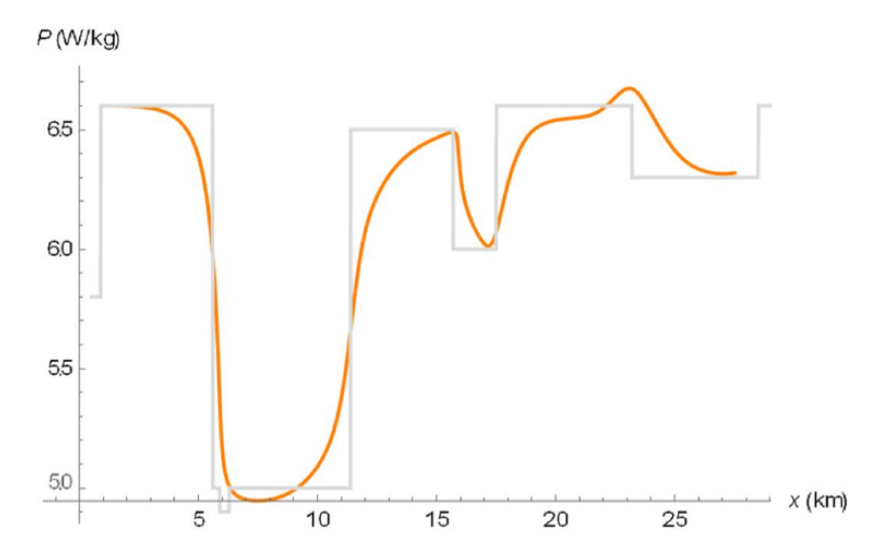
\includegraphics[width=\textwidth]{figures/image13.png}
    \caption{ Actual output power}
    \label{fig:image13}
  \end{minipage}\hfill
  \begin{minipage}{0.45\textwidth}
    \centering
    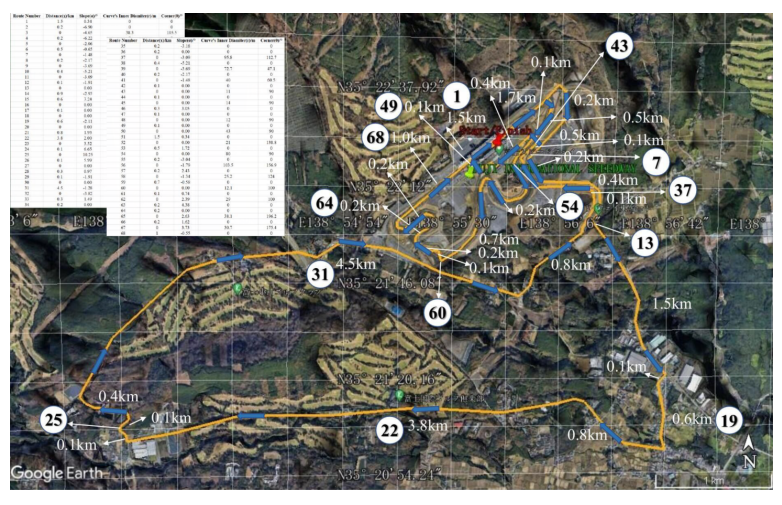
\includegraphics[width=\textwidth]{figures/image14.png}
    \caption{2021 Olympic track division}
    \label{fig:image14}
  \end{minipage}
\end{figure}
\subsection{The Strategy of 2021 Olympic Time Trial course}
As can be seen from fig.\ref{fig:image14}, the Tokyo Circuit is located near the city of Toyama, which is
surrounded by the treacherous Northern Alps Tateyama Mountains on three sides. The terrain here

changes greatly and the turns are sharp, which is significantly different from the Belgian track. This
event had high requirements on the slope skills of the cyclists. Besides, male cyclists need to circle
the track twice while female cyclists only need once.
We divided the Tokyo circuit into 68 segments and 2 zones (large circle and small circle) based
on the terrain and ramp characteristics of the area. The division situation is shown in fig. 14. Among
them, most road sections in the large circle and some sections in the small circle can still be calculated
by the previous model. For the other two road sections (the \#24-27 big climbing curve in fig. 16 and
the \#55-56 sharp curve in fig. 17), we will analyze them separately later.


\subsubsection{The Strategy for Regular Road Sections in Japan}

Based on our segmentation of the track, in the remaining 62 regular road segments,
$n_i=20$, $n_j=25$, $n_k=17$. Because $1-\cos2^\circ<7\times10^{-4}$ and
$\cos2^\circ-\cos4^\circ<2\times10^{-3}$, we apply the weighted-simplification 
method in section~5.4 to the slopes whose angle satisfies $\theta<2^\circ$ and 
$2^\circ<\theta<4^\circ$ respectively. The set of road-segment numbers that
meet the conditions is $\mathcal{T}_{U2}$, $\mathcal{T}_{D2}$, $\mathcal{T}_{U4}$,
$\mathcal{T}_{D4}$, with cardinalities $|\mathcal{T}_{U2}|=8$, $|\mathcal{T}_{D2}|=9$, $|\mathcal{T}_{U4}|=9$, $|\mathcal{T}_{D4}|=11$.
Ultimately, the problem transforms into the following nonlinear-programming problem:
\begin{align}
t &= \sum_{i=1}^{n_i} \frac{L_i}{v^{(straight)}(P_i)} + \sum_{j \notin I'D} \frac{D_j}{v_{\theta_j}^{(downhill)}(P_j)} + \sum_{k \notin I'U} \frac{U_k}{v_{\theta_k}^{(uphill)}(P_k)} + \sum_{rU,rD} \frac{U_{T_i}}{v_{\theta_{T_i}}^{(up/down)}(P_{T_i})} \notag \\
&\quad \text{as} \quad t = \Sigma_i + \Sigma_j + \Sigma_k + \Sigma_T \notag \\
&\qquad\qquad \text{find} \ P_{out}(t), \tag{17} \\
&\min \{t\} \quad s.t. \int_0^{t_n} \frac{dt^*}{T(P_{out}(t^*))} = 0.95 \notag
\end{align}

where $\varSigma_T$ represents the integrated-item term.

With the help of \textit{Mathematica}, we obtain the curve of $P_{\text{out}}(x)$, and the result is shown in fig.~15. Compared with 2021 UCI, the Tokyo circuit is more complicated; the difficulty of the riders' power-distribution strategy has also increased significantly.
\vspace{-0.5cm}
\begin{figure}[H]
  \centering
  \begin{subfigure}{0.45\textwidth}
    \centering
    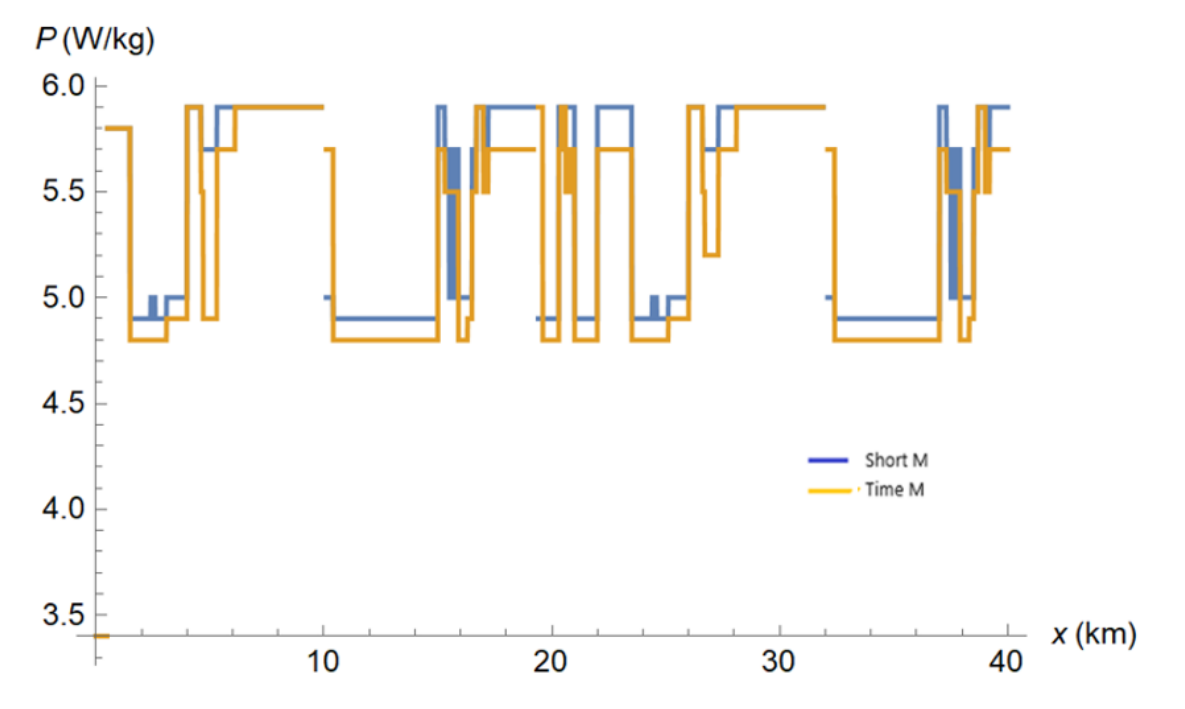
\includegraphics[width=\textwidth]{figures/image15_1.png}
    \caption{The $P_{out}(x)$ plot of male cyclist.}
    \label{fig:image15.1}
  \end{subfigure}\hfill
  \begin{subfigure}{0.45\textwidth}
    \centering
    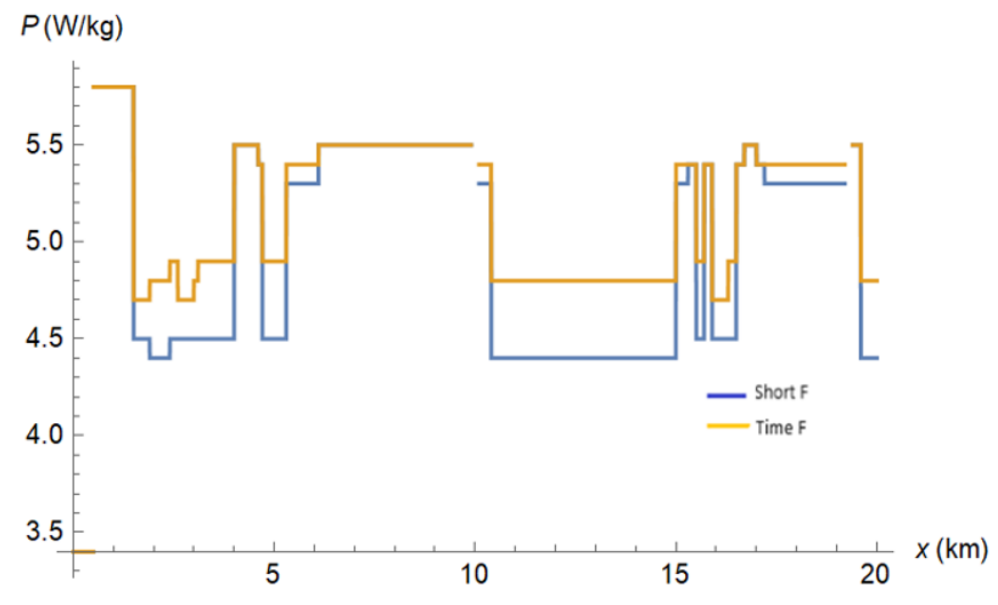
\includegraphics[width=\textwidth]{figures/image15_2.png}
    \caption{ The $P_{out}(x)$ plot of female cyclist. (The discontinuous part is a special road section and
needs to be solved separately)}
    \label{fig:image15.2}
  \end{subfigure}
  \caption{The result of 2021 Olympic Time Trial course}
\end{figure}
\begin{figure}[H]
    \centering
    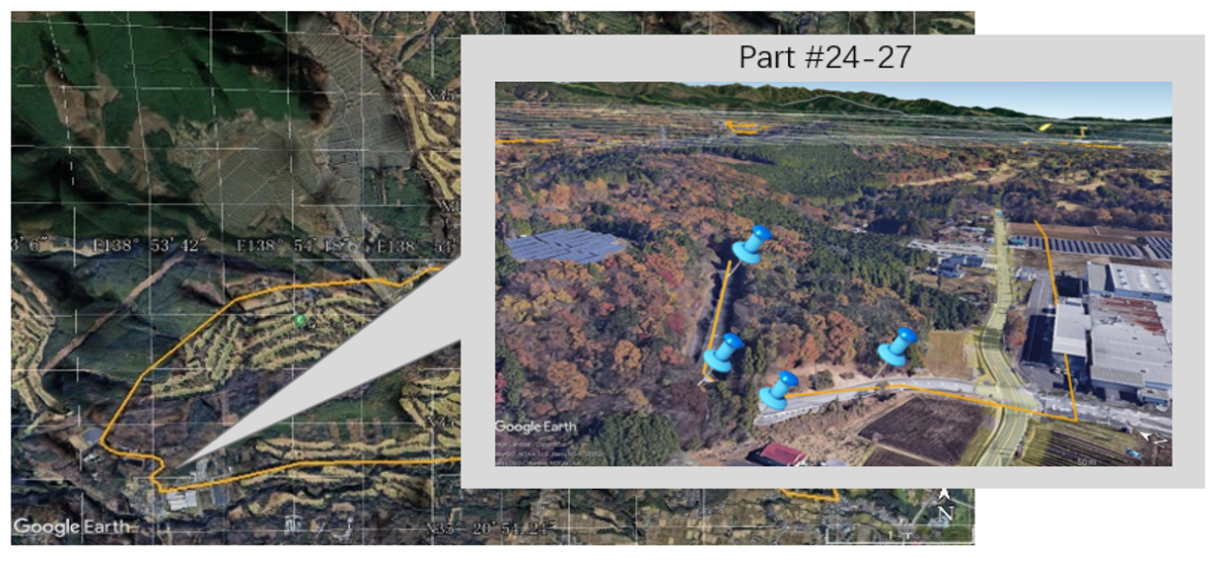
\includegraphics[width=0.8\textwidth]{figures/image16.png}
    \caption{Detail of section \#24-27}
\end{figure}
\subsubsection{The Strategy for Special Road Sections in Japan}

\textbf{(1)Huge hill turn of section \#24-27}


The parameters of these four sections are shown in the table below:
\begin{table}[H]
\centering
\caption{The data of section \#24-27}
\begin{tabular}{ccccc}
\hline
Section & Length & Turning radius & Slope angle & Turning angle \\
\hline
\#24 & 0.1km & 0m & $6.65°$ & $0°$ \\
\#25 & $\approx 0$km & 9m & $10.25°$ & $147°$ \\
\#26 & 0.1km & 0m & $5.99°$ & $0°$ \\
\#27 & $\approx 0$km & 8.5m & $4.22°$ & $79°$ \\
\hline
\end{tabular}
\end{table}

The straight part here is steep, such as section \#63 with a slope angle of $4.4°$. The cyclist speed here is 6.83m/s and the output power is 5.5W/kg. We will base our straights strategy around this data.

Next, we analyze the turning strategy. The curve is a sharp turn with continuous climbing. We use formula (*) to calculate. The best turning speed of section\#25 is $6.0m/s$, with $P^{(\#25)} = 6.32\ W/kg$. And the speed of section\#27 is $6.4\ m/s$, $P_{\max}^{(\#27)} = 5.31\ W/kg$. In this way, the time used for this section is 31.2s.

\textbf{Sharp turn of section\#55-56}

The parameters of these four sections are shown in the table below:
\begin{table}[H]
\centering
\caption{The data of section \#55-56}
\begin{tabular}{ccccc}
\hline
Section & Length & Turning radius & Slope angle & Turning angle \\
\hline
\#55km & 0.2m & $0°$ & $\approx 0°$ & $0°$ \\
\#56km & $\approx 0$m & $12°$ & $\approx 0°$ & $166.9°$ \\
\hline
\end{tabular}
\end{table}

As for this turn, it has a small inner diameter and a high turning angle of $166.9°$. By calculation,
$v_{\max}^{(\#56)} = 5.806\ m/s$, $P_{\max}^{(\#56)} = 4.32\ W/kg$. On the straight \#55, $P_{out} = 5.6\ W/kg$, $v = 10.0m/s$. We plan to start decelerating 20m before the start of section \#56. And accelerate back to the original speed immediately after passing the turn \#56. It take 21.7s.
\begin{figure}[H]
    \centering
    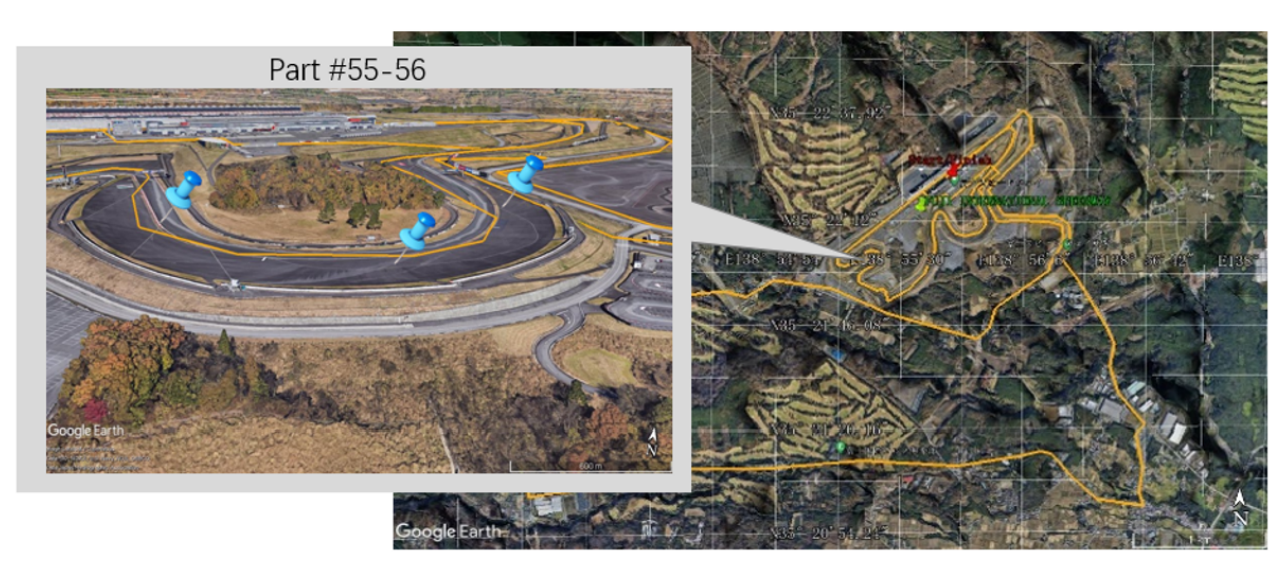
\includegraphics[width=0.8\textwidth]{figures/image17.png}
    \caption{Detail of section \#55-56}
\end{figure}
Combining 5.5.1 and 5.5.2, the results of the four players under the optimization strategy are
shown in the following table:
\begin{table}[H]
\centering
\caption{The results of 2021 Olympic Time Trial course}
\small
\begin{tabular}{lcccc}
\hline
Rider type & Male sprinter & Female sprinter & \makecell{Male time \\ trial specialist} & \makecell{Female time \\ trial specialist} \\
\hline
Complete time & 62.68min & 56.03min & 40.97min & 33.63min \\
\hline
\end{tabular}
\end{table}

It can be seen that the nontrivial road condition increases the test of the cyclist’s climbing
ability and endurance. The sprinter’s performance was significantly lower than that of the time trial
specialist. This disparity is larger than that of UCI.




\section{Sensitivity Analysis}
\subsection{Sensitive Analysis of Weather}
Weather conditions include temperature, humidity, wind speed, wind direction, etc.
According to the theory of blood CK and HB \cite{Ji2011TemperatureHumidity}, within a certain range, temperature and
humidity have little effect on the physical fitness of athletes. From Assumption 1, the conclusion can
be further proved reasonable.

Secondly, rain has little effect on the rolling friction coefficient of the asphalt track. Rain only
increases the demands on the driver’s turning skills. The literature \cite{Westlake2016RainSpeed} indicates that the negative
impact of rain can be eliminated to a certain extent through training.
In conclusion, our analysis of the sensitivity to weather factors will focus on wind speed and
direction.
We divide the sensitivity analysis into two parts: straight sections and turning sections to
determine the potential impact of wind directions and wind. The influence of the road gradient is
mainly reflected in the friction of the bicycle. Therefore, we uniformly assume that the road slope is
0\% in the sensitivity analysis.

\textbf{(1)Straight sections}


On the straights, only the effective wind speed will affect the ride. The effective wind speed is in
the same direction as the cyclist. Therefore, we only analyze the sensitivity of the model to the wind
speed in this part.
According to the wind speed requirements of cycling events, as well as the average wind speed
of Japan and Belgium in July, we selected the wind speed to be around 2m/s for analysis.
We use Python to draw the maximum output power curve and the wind resistance influence power
curve within the range of ±1\% deviation of wind speed. The results are shown in fig. \ref{fig:image18}.


\begin{figure}[ht]
  \centering
  \begin{minipage}{0.45\textwidth}
    \centering
    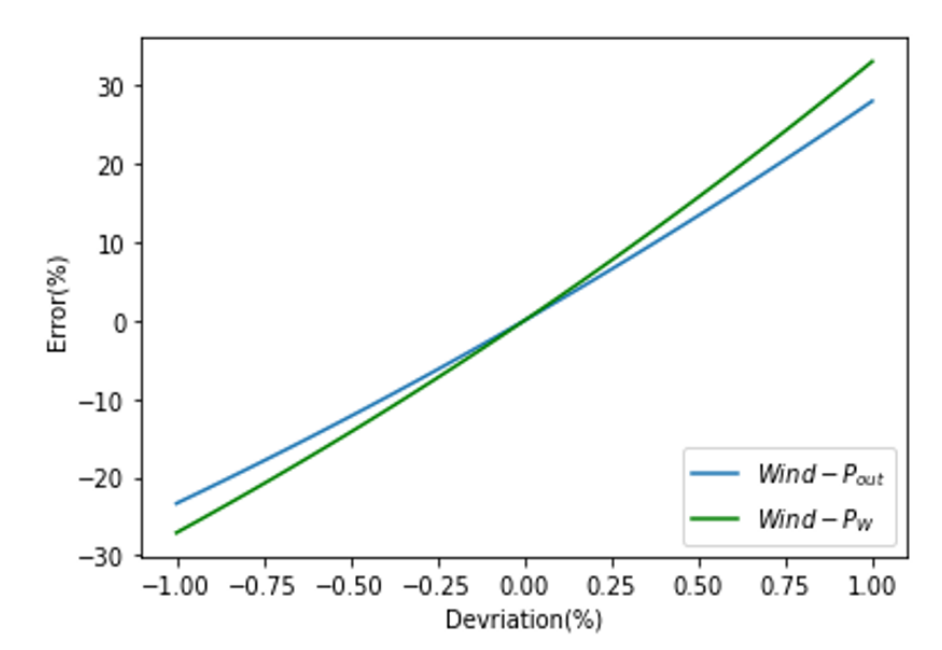
\includegraphics[width=\textwidth]{figures/image18.png}
    \caption{Sensitivity of wind speed}
    \label{fig:image18}
  \end{minipage}\hfill
  \begin{minipage}{0.45\textwidth}
    \centering
    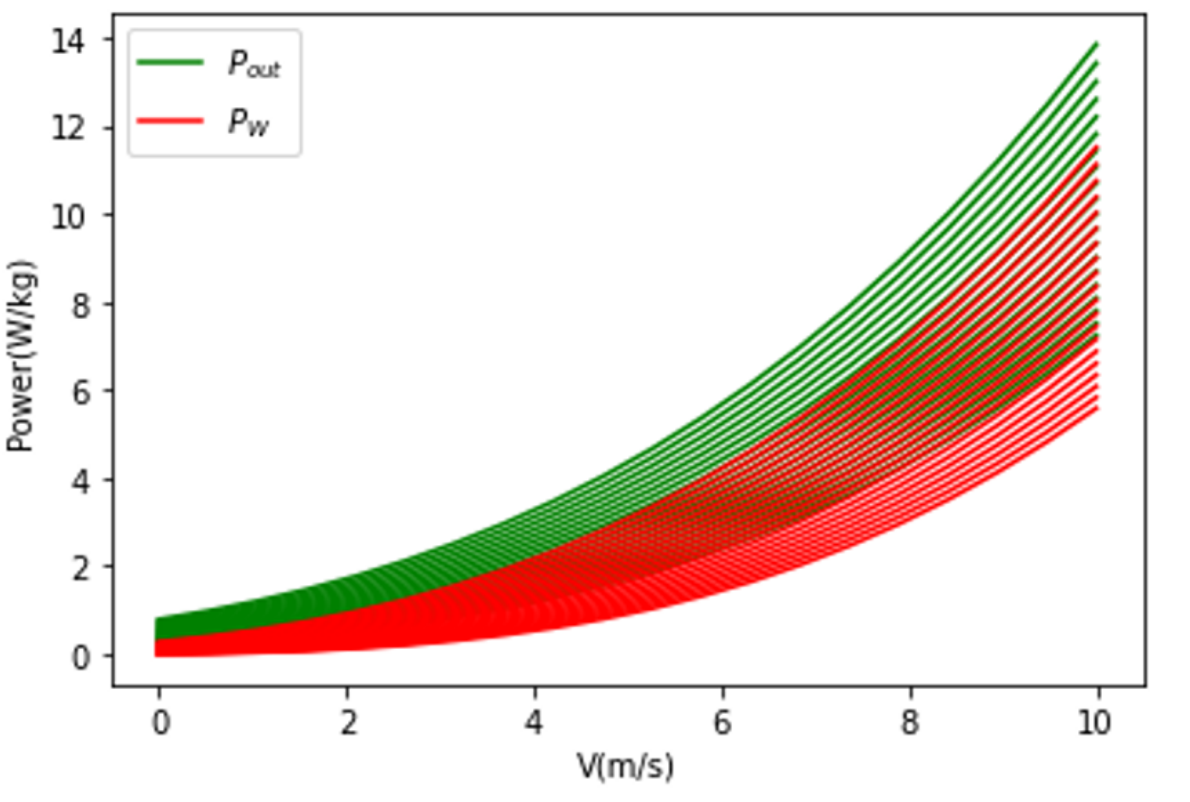
\includegraphics[width=\textwidth]{figures/image19.png}
    \caption{Change of $P_{out}(v)$ and $P_{W}(v)$}
    \label{fig:image19}
  \end{minipage}
\end{figure}
Figure \ref{fig:image19} shows the changes of and curves (moving from bottom to top) when the wind speed
changes from $1m/s$ to $4m/s$.
From the figure, when the cyclist rides at a constant speed on the straight, the deviation is 10\%.
Therefore, the model is more sensitive to wind speed in straight sections.

\textbf{(2)Turning sections}

Next, we analyze the model's sensitivity to wind speed and direction during turning. We use \textit{Python} to perturb the model within 10\% of the deviation from the wind speed and direction. The results are shown in fig. 20. where $\gamma$ is the local wind angle.

During the turning sections, the effect of wind direction change on the rider's maximum output power is on the order of 0.1\%, while the effect of wind speed changes is on the order of 0.01\%. Both effects are much smaller than the straight sections. Therefore, the model is less sensitive to wind speed and direction in the turning sections.

In conclusion, the change of wind direction and speed within a certain range will not affect the turning strategy of the model. On the other hand, the model is more sensitive to headwind. In individual races, the output power when the wind is down can be appropriately reduced, while the wind is up it can be increased.
\begin{figure}[ht]
    \centering
    \begin{minipage}{0.45\textwidth}
        \centering
        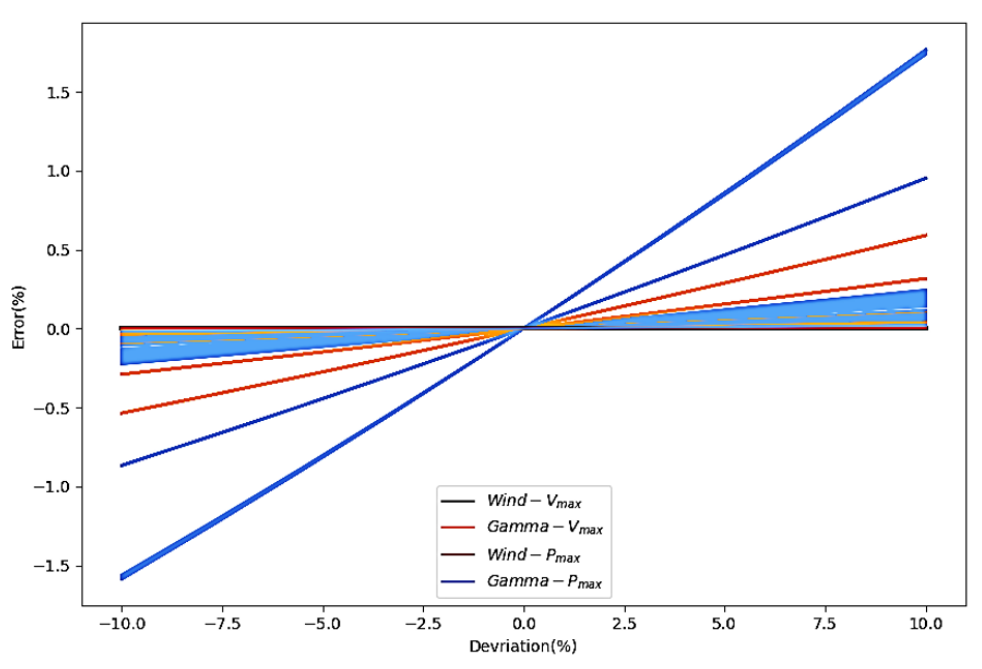
\includegraphics[width=\textwidth]{figures/image20_1.png}
    \end{minipage}\hfill
    \begin{minipage}{0.45\textwidth}    
        \centering
        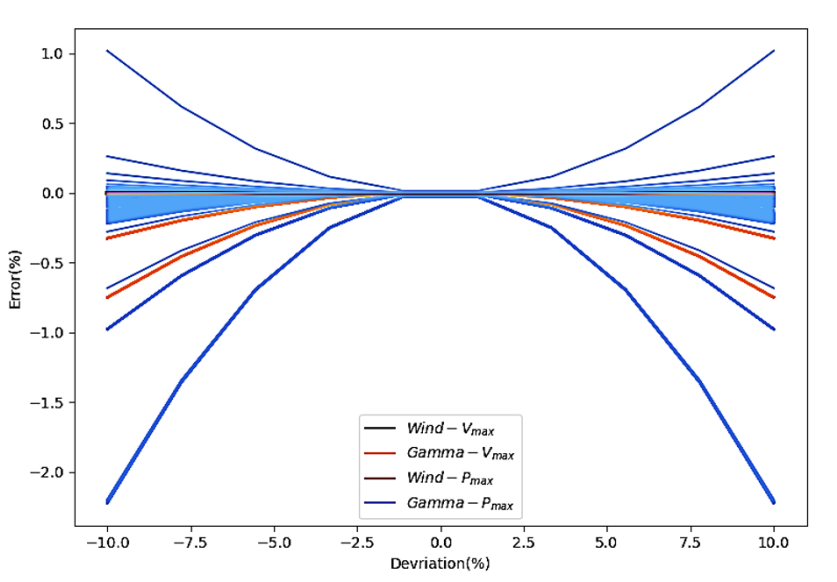
\includegraphics[width=\textwidth]{figures/image20_2.png}
    \end{minipage}
\caption{Sensitivity of wind speed\&direction. Left: The course in Japan, with $v_{\text{wind}} = 2\,\text{m/s}$, $\gamma = -45°$. Right: The course in Belgium, with $v_{\text{wind}} = 2\,\text{m/s}$, $\gamma = 180°$.}
\label{fig:20}
\end{figure}

In addition, this phenomenon provides ideas for the strategy of team time trial, which we will
focus on in Section VII.

\subsection{Sensitive Analysis of Rider Deviations}

In the $P_{\text{out}}(x)$ solution process of 5.3--5.5, we adopt an idealized approximate discrete value model, so the power output of the rider on each small segment remains constant. In practical situations, due to the randomness of the rider's operation, it is difficult to strictly follow the optimal power curve. In this part we will test the sensitivity of the rider deviations from the target power to the model.

First, take the time trial in the 2021 UCI as an example.
We perform spline interpolation on each segment of the
discrete $P_{\text{out}}(x)$ based on its endpoint values.
They are then used as a function $P_{\text{out}}$ of the 
actual output of the rider. Then, we add random disturbance term 
$\widetilde{{P}_{\text{out}}} = \sum_{i=1}^{4} A_i \sin(0.1i \cdot t)$,
where $A_i$ is determined by a random number and 
$0 < A_i < 5\% \cdot P_{\text{out}}^{(\text{max})}$. 
Then the actual power output function of the rider is 
$P_{\text{out}}^{(\text{real})} = \widetilde{{P}_{\text{out}}} + \overline{P}_{\text{out}}$. 
We conduct three experiments and get three
 $P_{\text{out}}^{(\text{real})}(x)$ curves.
 Plot them in the same coordinate system as the ideal
  $P_{\text{out}}(x)$ curve, as shown in the left of fig. \ref{fig:image21}.
\begin{figure}[ht]
    \centering
    \begin{minipage}{0.4\textwidth}
        \centering
        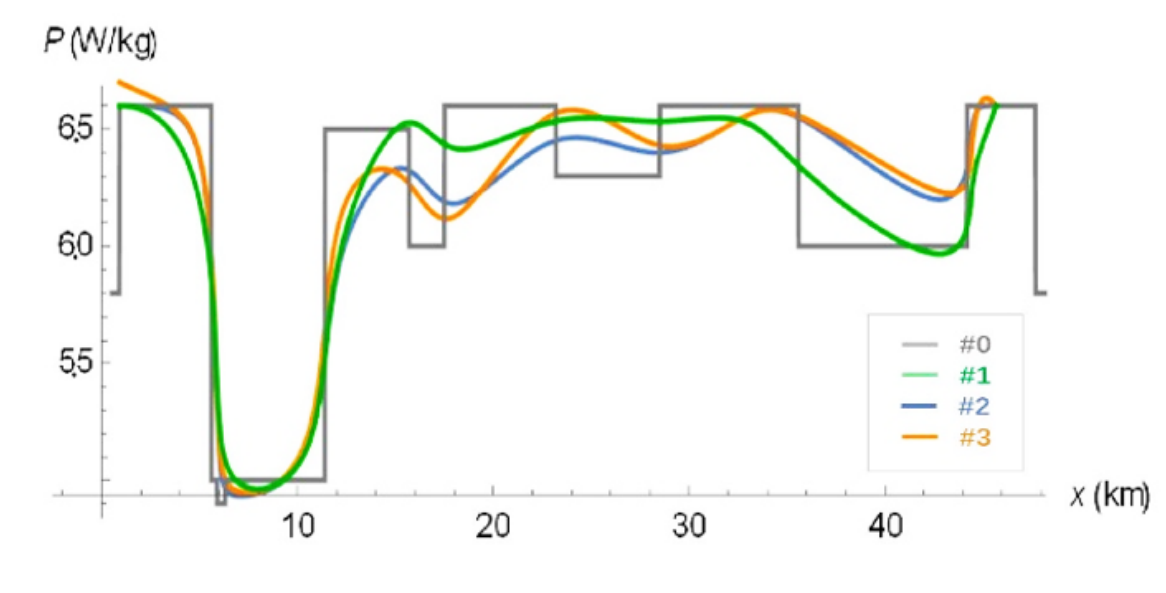
\includegraphics[width=\textwidth]{figures/image21_1.png}
    \end{minipage}\hfill
    \begin{minipage}{0.3\textwidth}    
        \centering
        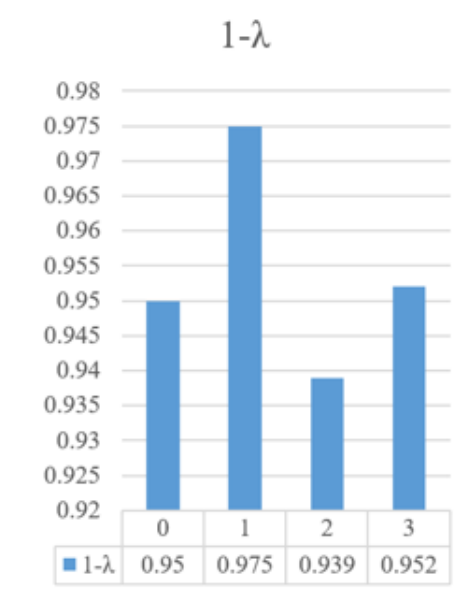
\includegraphics[width=\textwidth]{figures/image21_2.png}
    \end{minipage}\hfill
    \begin{minipage}{0.3\textwidth}
        \centering
        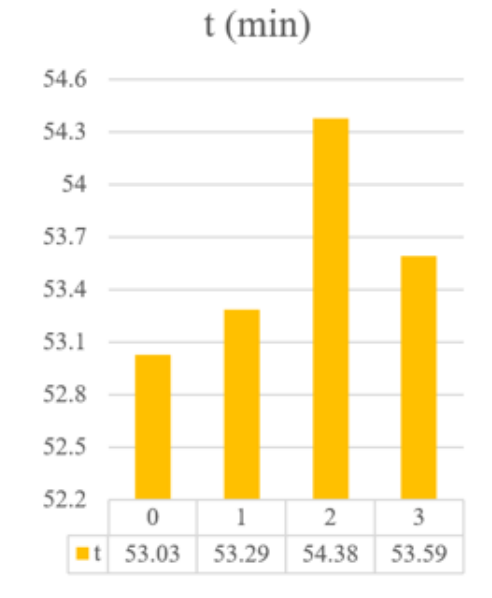
\includegraphics[width=\textwidth]{figures/image21_3.png}
    \end{minipage}
\caption{The results of the model. Left: The curve of $P_{\text{out}}(x)$ \& $P_{\text{out}}^{(\text{real})}(x)$. Middle: 1- of different strategies. Right: The Competition time of different strategies}
  \label{fig:image21}
\end{figure}

We put the four curves into the energy constraints, and it turned out that all riders could finish the
race. In terms of whether it can finish the race, the stability of the model is excellent. The specific

results are shown in the middle of fig. \ref{fig:image21}.
Next, we calculated the time it took for the rider to reach the finish line (see the right of fig. \ref{fig:image21}).
Rider results are all below the ideal output curve. But the lag time is within 2.5\% of the optimal
time. Therefore, the sensitivity of the race performance to the actual strategy of the rider is low. We
recommend that riders maintain an ideal power curve at the end of each segment, which helps reduce
lag time.

Finally, we compared the calculation results of our model with the results of the actual competition
winners. The results are as follows:
\begin{table}[H]
\centering
\caption{The comparison between Championship results and our model's results}
\label{tab:11}
\begin{tabular}{ccc}
\hline
Rider type & Male cycling time trial & Female cycling time trial \\
\hline
The results of our model & 56.03 min & 34.63 min \\
Championship results & 55.08 min & 30.22 min \\
\hline
\end{tabular}
\end{table}

The model's results are slightly behind the world championship
 results. This may be related to the fact that the experimental 
 data samples we use to determine the power curve are from average
  riders rather than top riders.

Compared with the championship, the results of our model 
solution are reasonable. It also shows that our model has 
the effect of bringing average-qualified riders close to
 the performance of champion riders, which illustrates the
  effectiveness of the model.


\section{ Further Discussion of The Team Time Trial}
In the 6.1, we concluded that the crosswind have little effect on the rider, while the headwind have a big effect. We found that this feature can be applied to the optimization of team time trials. By reviewing the literature, we came to the following conclusions:

Due to the existence of drafting yields, within a certain distance ($<1\text{ m}$), the wind resistance of the second rider on the pace line is reduced to 60--70\% of the individual rider. While the drag for the third rider dropped to about 50--63\%. The drag along the convoy will gradually decrease to about 47--60\%.

In addition, due to the existence of ``subsonic upstream disturbance''. With multiple riders, it's not necessarily that the last rider has the least wind resistance. In fact, the last rider is the only rider on the pace line who didn't benefit from the subsonic upstream disturbance.

We will mainly analyze the formation strategy of the cycling team to deal with the headwind on the straight. We calculated the team and individual results on the 1 km straight to verify the rationality and effectiveness of the strategy.

For the 6-person cycling team, we have two formations, the snake and the pyramid. For the 4-person sprint cycling team, we designed the shield formation as shown in the left of fig. 22. The numbers in the heat map represent the ratio of the wind resistance of the individual in the team competition to that in the same state of the individual competition$C_f$.
\begin{figure}[H]
\centering
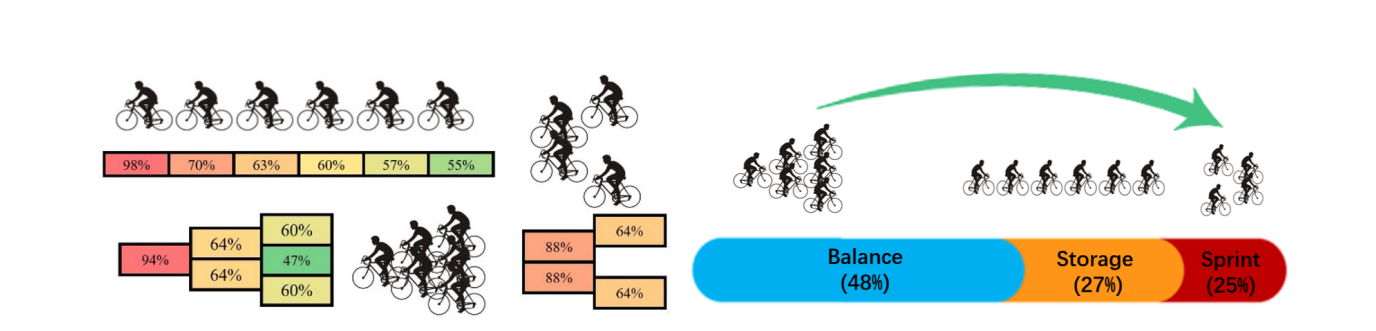
\includegraphics[width=0.8\textwidth]{figures/image22.png}
\caption{Left: Schematic diagram of three formations in team time trial. Right: Team strategy in
the time trial.}
\label{fig:image22}
\end{figure}
We divide the race into three stages to calculate the team race results on the 20 km straight: Balance, Storage, and Sprint. The lengths are $L_B$, $L_S$, $L_R$ and $L_B + L_S + L_R = 20\text{ km}$.

\begin{itemize}
\item \textbf{Balance:} 6 riders take turns riding in 6 positions. In this way, the physical energy consumption caused by wind resistance is balanced. We choose the formation with the lowest average resistance coefficient $K_f$ as the optimal one. It is calculated that the snake formation $K_f = 67.17$ and the pyramid formation $K_f = 64.83$, so we choose the pyramid formation.

\item \textbf{Storage:} Since changing the formation will cause the rider to consume excess physical strength; the formation should be maintained as much as possible. Besides, the four riders who cross the line should rotate in the position with the smaller drag coefficient, while the other two riders (called windbreakers) should rotate in the place with the larger drag coefficient. Considering the balance of the sprinters in the long snake formation, we choose the long snake formation after weighing.

\item \textbf{Sprint:} According to the simulation results of literature [12], we choose the shield formation with the smallest drag coefficient.
\end{itemize}

Next, take the data of male time trial specialists as an example to calculate. The result is that the Balance section accounts for 48\%, the Storage section accounts for 27\%, and the sprint section accounts for 25\%, as shown in Figure e2. The 20 km straight individual race was 24.8 min, and the team race was 21.2 min. The team competition results are significantly better than the individual competition. Compared with the average speed of the Tour de France 2018 Stage3 champion BMC team of 56.1 km/h, the average rate of our model on the straights is 56.6 km/h, proving the model's accuracy.
\begin{figure}[H]
    \centering
    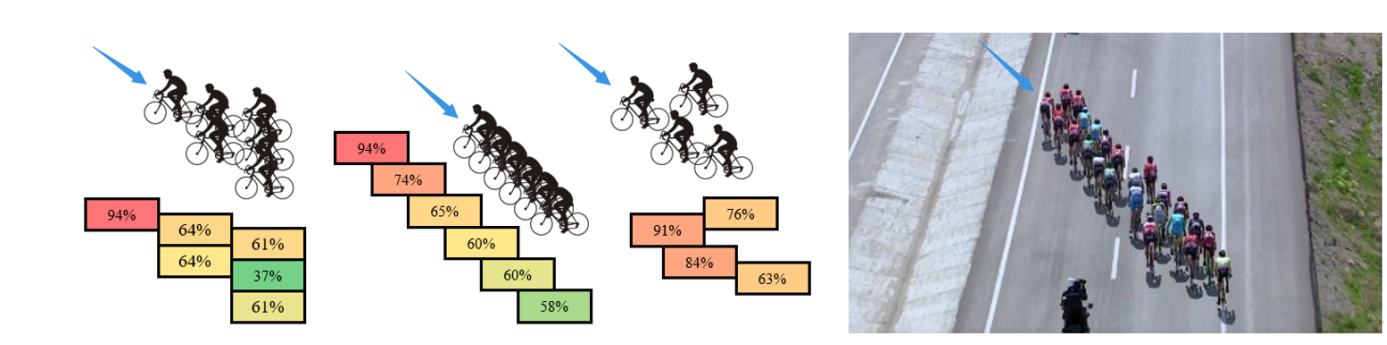
\includegraphics[width=0.8\textwidth]{figures/image23.png}
    \caption{ Left: Cycling strategy for lateral wind. Right: Slanted line array in Tour of Turkey 2016.}
    \label{fig:image23}
\end{figure}
In addition, for the case of crosswind, we take the wind coming from the right front as an example.
The formation should be adjusted to the diagonal array, as shown in fig. \ref{fig:image23}. It is beneficial to reduce
drag coefficient and reduce crosswind disturbance.
\section{Model Evaluation and Further Discussion}
\subsection{Strengths}
\begin{itemize}
\item \textbf{Efficient solutions}  We exploit the linearity or near-linearity of the function when solving
the optimal policy. The solution speed and convergence speed are greatly improved when
performing integration and discrete approximations.
\item \textbf{Accuracy of results} We relied on data and literature for model simplification. And we have
analyzed the special part of the track separately, which guarantees the accuracy. In addition,
the solution results of the model are close to the championship results, which verifies the
accuracy of the results.
\item \textbf{Universality }The piecewise nonlinear programming model we adopted is suitable for races
where track information and player information are known. In addition to cycling time trials,
swimming, running and other competitions can also be applied by modifying the parameters.
\item \textbf{Stability and high fault tolerance} Our model was tested for sensitivity and its stability was
verified. We chose the parameters of the average rider and set the energy utilization to 95\%.
These steps also improve the fault tolerance of the model.
\end{itemize}
\subsection{Weaknesses}
\begin{itemize}
\item \textbf{ Lack of adversary factor} Our model mainly analyzes unopposed time trials. The modeling
process lacks consideration of offense and defense strategies among riders.
\item  \textbf{Difficulty in further improving accuracy} We used numerical methods and discrete methods
in the model. These methods limit the accuracy of the model. So in Sections VI and VII, we
discuss the model further to improve this problem. It turns out that the improved model is
more accurate.
\end{itemize}
\subsection{Conclusion}
Our paper provides a detailed analysis of the relationship between riding strategy and power
curve. Before introducing our model, we analyze the characteristics of various types of riders and
different kinds of tracks. Then the three-stage power curve model and dynamic bicycle model are
proposed.

Next, in order to use the established mathematical model to optimize the strategy of the bicycle
time trial, we divide the complex track into several simple segments according to the track characteristics such as slope and turn. Then, using nonlinear programming to solve the optimal strategy,
we analyzed the self-made track, the Belgian track, and the Tokyo track. Different types and genders
of players have different strategies. For the Belgian track, the deviation of the model solution results
from the world championship results is about 8\%. The model results deviate by about 6\% for the
Tokyo circuit. After that, we analyzed the model’s sensitivity to weather factors and rider deviations.
Among the weather factors, wind speed and direction dominate. We conclude that the model is
more sensitive to headwind. This conclusion is beneficial to the formation analysis of the team time
trial. We perturbed the model with random disturbance terms when studying the sensitivity to rider
deviations, resulting in three power curves. The riders finish the race in this disturbance with little
difference in their time, proving our model’s robustness.
\nocite{*} 
\bibliographystyle{plain}   % 选用样式（plain / IEEEtran / elsarticle-harv ...）
\bibliography{reference}  
\end{document}